\documentclass{beamer}

\usepackage[T2A]{fontenc}
\usepackage[utf8x]{inputenc}
\usepackage[english,bulgarian]{babel}
\usepackage{multirow}
\usepackage{ragged2e}

\mode<presentation> {
	\usetheme{Berlin}
}

%\usebackgroundtemplate {
%	\includegraphics[width=370px, height=270px, trim=0 0 0 -80px]{background}
%}

\graphicspath{{../images/}}

\title{Статистическа обработка на данните}
\subtitle{Статистическа обработка на данни с R}

\author{Пламен Петров и Тодор Балабанов}

\date{5.VI.2020}

\institute[ЦО и ИИКТ към БАН] {
	Център за обучение \\
	Институт по информационни и комуникационни технологии \\ 
	Българската академия на науките \\
	\medskip
	\textit{p.petrov@iit.bas.bg todorb@iinf.bas.bg}
}

\addtobeamertemplate{navigation symbols}{}{
	\usebeamerfont{footline}
	\usebeamercolor[fg]{footline}
	\hspace{1em}
	\insertframenumber/\inserttotalframenumber
}

\begin{document}

\begin{frame}
	\titlepage
\end{frame}

\begin{frame}
\begin{exampleblock}{Acknowledgments}
\justify These teaching materials are funded by Velbazhd Software LLC and it is partially supported by the Bulgarian Ministry of Education and Science (contract D01–205/23.11.2018) under the National Scientific Program ``Information and Communication Technologies for a Single Digital Market in Science, Education and Security (ICTinSES)'', approved by DCM \# 577/17.08.2018.
\end{exampleblock}
\end{frame}

\section*{Теми}
\begin{frame}[shrink]
	\frametitle{Съдържание}
	\tableofcontents
\end{frame}

\section{Описателна статистика}

\begin{frame}
\center \huge{Описателна статистика}
\end{frame}

\subsection{Групиране и разпръскване}

\begin{frame}
\frametitle{Централно групиране на данните и разпръскване}
\begin{block}{Генериране на извадка от случайни числа}
v1 <- round( rnorm(100, mean=62, sd=72) )

v2 <- v1

v2[sample(x=1:100, size=15, replace=FALSE)] <- NA

w1 <- 1 / sample(x=1:100, size=100, replace=TRUE)
\end{block}
\end{frame}

\begin{frame}
\frametitle{Най-често използвана централна статистика}
\begin{block}{Средна стойност}
sum(v1) / length(v1)

mean( v1 )

mean( v2 )

mean(v2, na.rm=TRUE)
\end{block}

\begin{block}{Претеглена средна стойност}
weighted.mean(x=v1, w=w1)
\end{block}
\end{frame}

\begin{frame}
\frametitle{Минимум, максимум, медиана и мода}
\begin{block}{Гранични статистики}
min( v1 )

max( v1 )
\end{block}

\begin{block}{Други централни статистики}
median( v1 )

unique(v1)[ which.max( tabulate(match(v1,unique(v1)) ) ) ]
\end{block}
\end{frame}

\begin{frame}
\frametitle{Статистики за разпръскване}
\begin{block}{Дисперсия и стандартно отклонение}
sum( (v1-mean(v1))\textasciicircum 2 ) / (length(v1) - 1)

var( v1 )

sqrt( var(v1) )

sd( v1 )
\end{block}
\end{frame}

\begin{frame}
\frametitle{Разпределяне по проценти}
\begin{block}{Квантили и обобщение}
quantile(v1, probs=c(0.1, 0.2, 0.3, 0.4, 0.5, 0.6, 0.7, 0.8, 0.9))

summary( v1 )
\end{block}
\end{frame}

\section{Сравнителна статистика}

\begin{frame}
\center \huge{Сравнителна статистика}
\end{frame}

\subsection{Корелация и ковариация}

\begin{frame}
\frametitle{Търсене на взимни връзки}
\begin{block}{Корелация между две променливи}
cor(economics\$psavert, economics\$pce)

sum((economics\$psavert-mean(economics\$psavert)) * (economics\$pce-mean(economics\$pce))) / ((nrow(economics)-1) * sd(economics\$psavert) * sd(economics\$pce))

cor(economics[, c($"$pce$"$, $"$psavert$"$, $"$uempmed$"$, $"$unemploy$"$)])
\end{block}
\end{frame}

\begin{frame}
\frametitle{Търсене на взимни връзки}
\begin{block}{Ковариация между две променливи}
cov(economics\$psavert, economics\$pce)

cov(economics[, c($"$pce$"$, $"$psavert$"$, $"$uempmed$"$, $"$unemploy$"$)])

identical(cov(economics\$psavert, economics\$pce), cor(economics\$psavert, economics\$pce) * sd(economics\$psavert) * sd(economics\$pce))
\end{block}
\end{frame}

\begin{frame}
\frametitle{Корелационен коефициент}
\begin{equation}
r_{xy} = \frac{\sum_{i=1}^{n}(x_i-\bar{x})(y_i-\bar{y})}{(n-1)s_xs_y}
\end{equation}
\end{frame}

\begin{frame}
\frametitle{Ковариационен коефициент}
\begin{equation}
v_{xy} = \frac{1}{n-1}\sum_{i=1}^{n}(x_i-\bar{x})(y_i-\bar{y})
\end{equation}
\end{frame}

\subsection{Тест на Стюдънт}

\begin{frame}
\frametitle{Сравнения на параметри}
\begin{block}{}
library(reshape2)
\end{block}

\begin{block}{Тест на единична извадка}
t.test(tips\$tip, alternative=$"$two.sided$"$, mu=3.50)
\end{block}

\begin{block}{Едностранна t-статистика}
t.test(tips\$tip, alternative=$"$less$"$, mu=3.50)
\end{block}
\end{frame}

\begin{frame}
\frametitle{T-статистика}
\begin{equation}
t = \frac{\bar{x}-\mu_0}{s_{\bar{x}}/\sqrt{n}}
\end{equation}
\end{frame}

\begin{frame}
\frametitle{Т-статистика за бакшиши}
\begin{figure}[]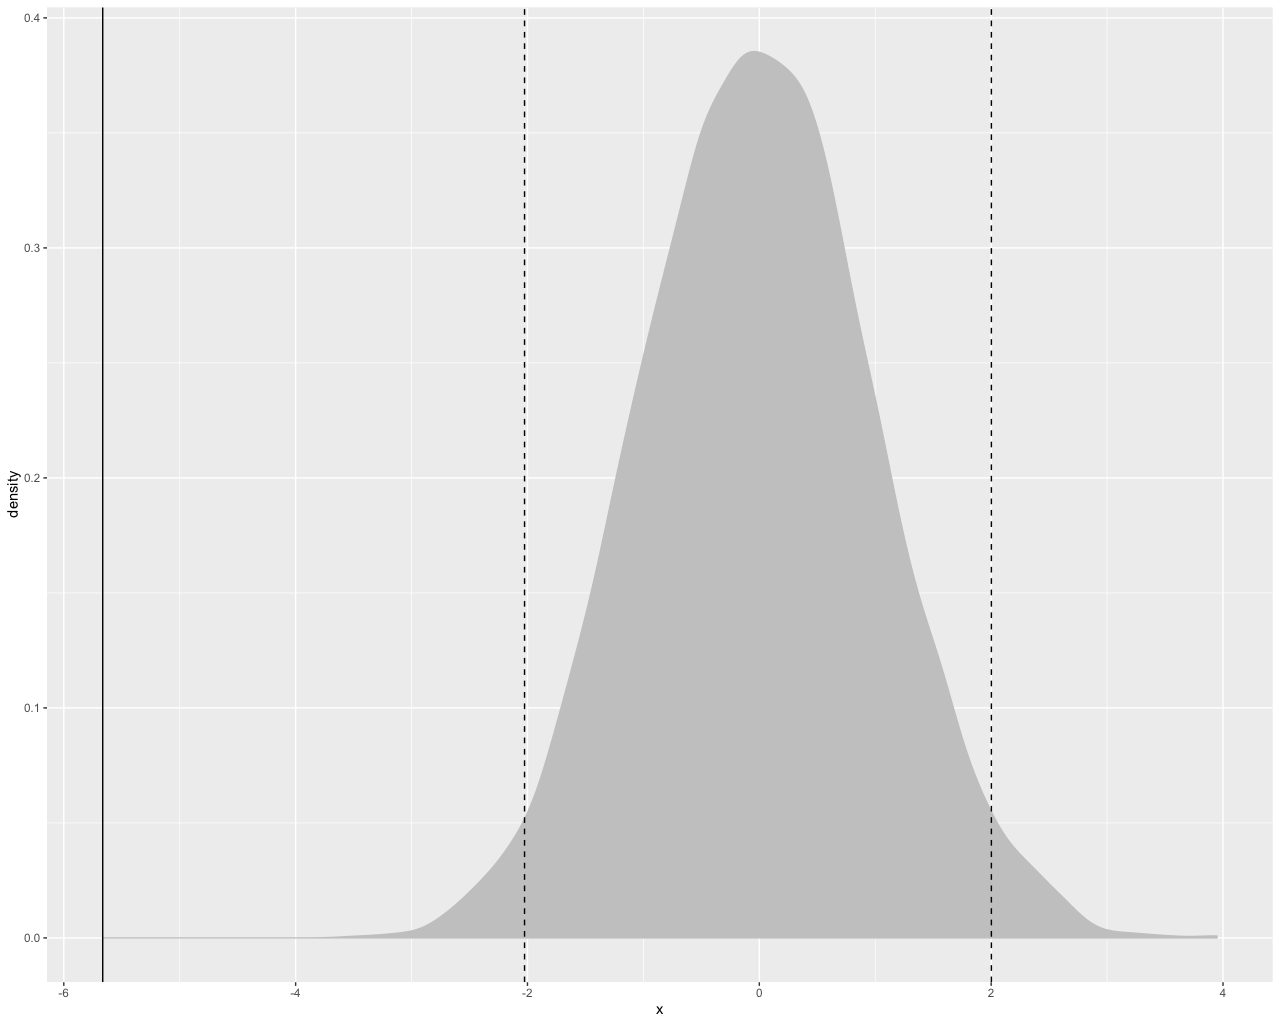
\includegraphics[width=\textwidth,height=0.75\textheight]{pic0056}\end{figure}
\end{frame}

\begin{frame}
\frametitle{}
\begin{block}{Визуализация на t-разпределение}
library( ggplot2 )

values <- rt(10000, df = NROW( tips ) - 1)

t <- t.test(tips\$tip, alternative=$"$two.sided$"$, mu=3.50)

ggplot(data.frame(x=values)) + geom\_density(aes(x=x), fill=$"$grey$"$, color=$"$grey$"$) + geom\_vline(xintercept=t\$statistic) + geom\_vline(xintercept=mean(values) + c(-2, 2) * sd(values), linetype=2)
\end{block}
\end{frame}

\subsubsection{Тест на две извадки}

\begin{frame}
\frametitle{Сравнение на две извадки}
\begin{block}{С прилагане на тест за нормално разпределение}
ggplot(tips, aes(x=tip, fill=sex)) + geom\_histogram(binwidth=1.0, alpha=0.8)

aggregate(tip\textasciitilde sex, data=tips, var)

shapiro.test(tips\$tip[tips\$sex == $"$Female$"$])

shapiro.test(tips\$tip[tips\$sex == $"$Male$"$])

shapiro.test( tips\$tip )

ansari.test(tip\textasciitilde sex, tips)

t.test(tip\textasciitilde sex, data=tips, var.equal=TRUE)
\end{block}
\end{frame}

\begin{frame}
\frametitle{Сравнения на параметри}
\begin{block}{Визуализация на двете извадки}
library( plyr )

ddply(tips, $"$sex$"$, summarize, tip.mean=mean(tip), tip.sd=sd(tip), Lower=tip.mean-2*tip.sd/sqrt(NROW(tip)), Upper=tip.mean+2*tip.sd/sqrt(NROW(tip))) 

ggplot(ddply(tips, $"$sex$"$, summarize, tip.mean=mean(tip), tip.sd=sd(tip), Lower=tip.mean-2*tip.sd/sqrt(NROW(tip)), Upper=tip.mean+2*tip.sd/sqrt(NROW(tip))), aes(x=tip.mean, y=sex)) + geom\_point() + geom\_errorbarh(aes(xmin=Lower, xmax=Upper), height=.2)
\end{block}
\end{frame}

\begin{frame}
\frametitle{Разпределение на бакшишите според пола на сервитьора}
\begin{figure}[]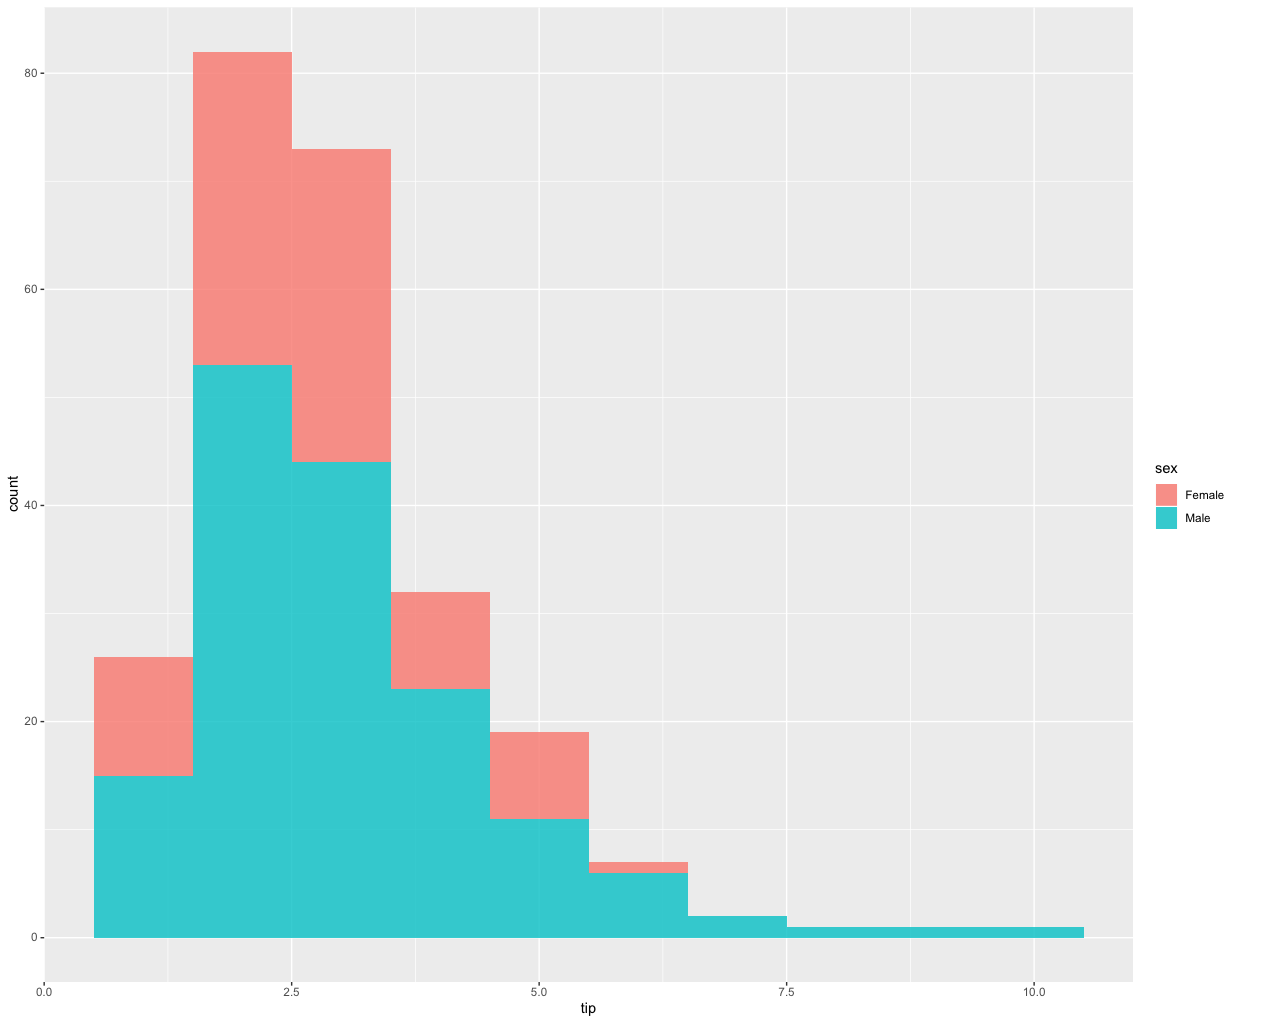
\includegraphics[width=\textwidth,height=0.75\textheight]{pic0057}\end{figure}
\end{frame}

\subsubsection{Сдвоен тест на две извадки}

\begin{frame}
\frametitle{Сравнение по двойки}
\begin{block}{Т-тест на сдвоени данни}
library( UsingR )

t.test(father.son\$sheight, father.son\$fheight, paired=TRUE)
\end{block}

\begin{block}{Визуализация}
ggplot(father.son, aes(x=fheight-sheight)) + geom\_density() + geom\_vline(xintercept=mean(father.son\$fheight-father.son\$sheight)) + geom\_vline(xintercept = mean(father.son\$fheight-father.son\$sheight) + 2*c(-1, 1 ) *sd(father.son\$fheight-father.son\$sheight)/sqrt(nrow(father.son)), linetype=2)
\end{block}
\end{frame}

\begin{frame}
\frametitle{Визуализация на средните при сдвоения тест}
\begin{figure}[]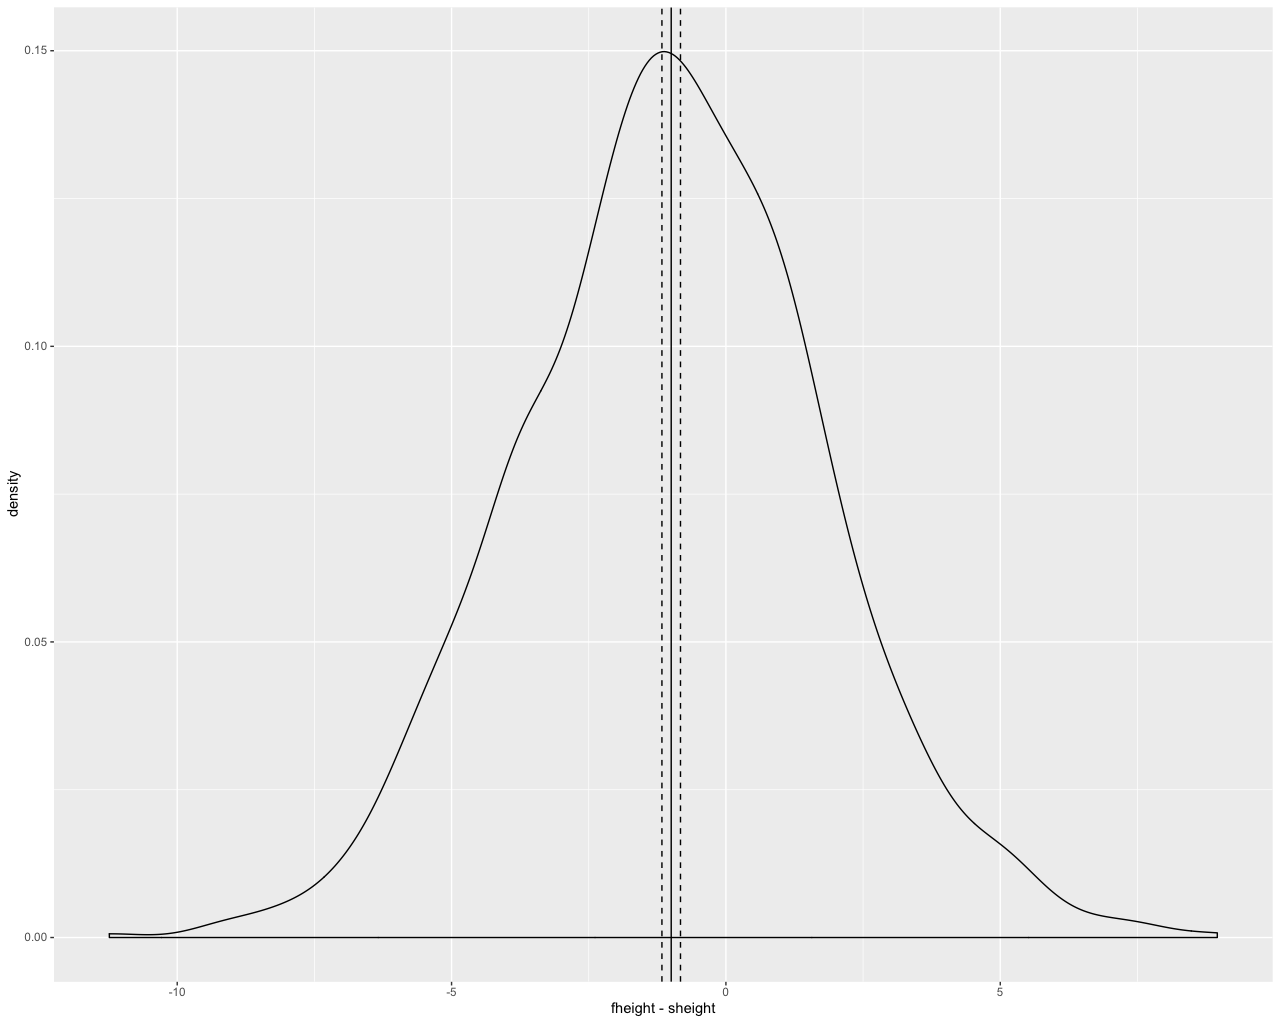
\includegraphics[width=\textwidth,height=0.75\textheight]{pic0058}\end{figure}
\end{frame}

\section{Дисперсионен анализ}

\begin{frame}
\center \huge{Дисперсионен анализ}
\end{frame}

\subsection{Сравнение при повече от две групи данни}

\begin{frame}
\frametitle{F-статистика за ANOVA}
\begin{equation}
F = \frac{ \sum_{i}^{}n_i(\bar{Y_i}-\bar{Y})^2 / (K-1) }{ \sum_{ij}^{}(Y_{ij}-\bar{Y_i})^2 / (N-K) }
\end{equation}
\end{frame}

\begin{frame}
\frametitle{Сравнение на дисперсиите}
\begin{block}{ANOVA тест}
library( plyr )

library( reshape2 )

aov(tip\textasciitilde day-1, tips)

aov(tip\textasciitilde day-1,tips)\$coefficients

summary( aov(tip\textasciitilde day-1,tips) )

ddply(tips, $"$day$"$, plyr::summarize, tip.mean=mean(tip), tip.sd=sd(tip), Length=NROW(tip), tfrac=qt(p=.90, df=Length-1), Lower=tip.mean - tfrac*tip.sd/sqrt(Length), Upper=tip.mean + tfrac*tip.sd/sqrt(Length))

summary( lm(tip\textasciitilde day-1,data=tips) )
\end{block}
\end{frame}

\section{Линейна регресия}

\begin{frame}
\center \huge{Линейна регресия}
\end{frame}

\subsection{Формули на линейната регресия}

\begin{frame}
\frametitle{Уравнение, наклон и срез на права}
\begin{equation}
y = ax + b + \epsilon
\end{equation}

\begin{equation}
a = \frac{ \sum_{i=1}^{n}(x_i-\bar{x})(y_i-\bar{y}) }{ \sum_{i=1}^{n}(x_i-\bar{x})^2 }
\end{equation}

\begin{equation}
b = \bar{y} - a
\end{equation}
\end{frame}

\begin{frame}
\frametitle{Изчисление на леинейна регресия}
\begin{block}{Наклон и срез}
library(ggplot2)

library(UsingR)

ggplot(father.son, aes(x=fheight, y=sheight)) + geom\_point() + geom\_smooth(method=$"$lm$"$) + labs(x=$"$Fathers$"$, y=$"$Sons$"$)

lm(sheight\textasciitilde fheight, data=father.son)

summary( lm(sheight\textasciitilde fheight,data=father.son) )
\end{block}
\end{frame}

\begin{frame}
\frametitle{Линейна регресия бащи-синове}
\begin{figure}[]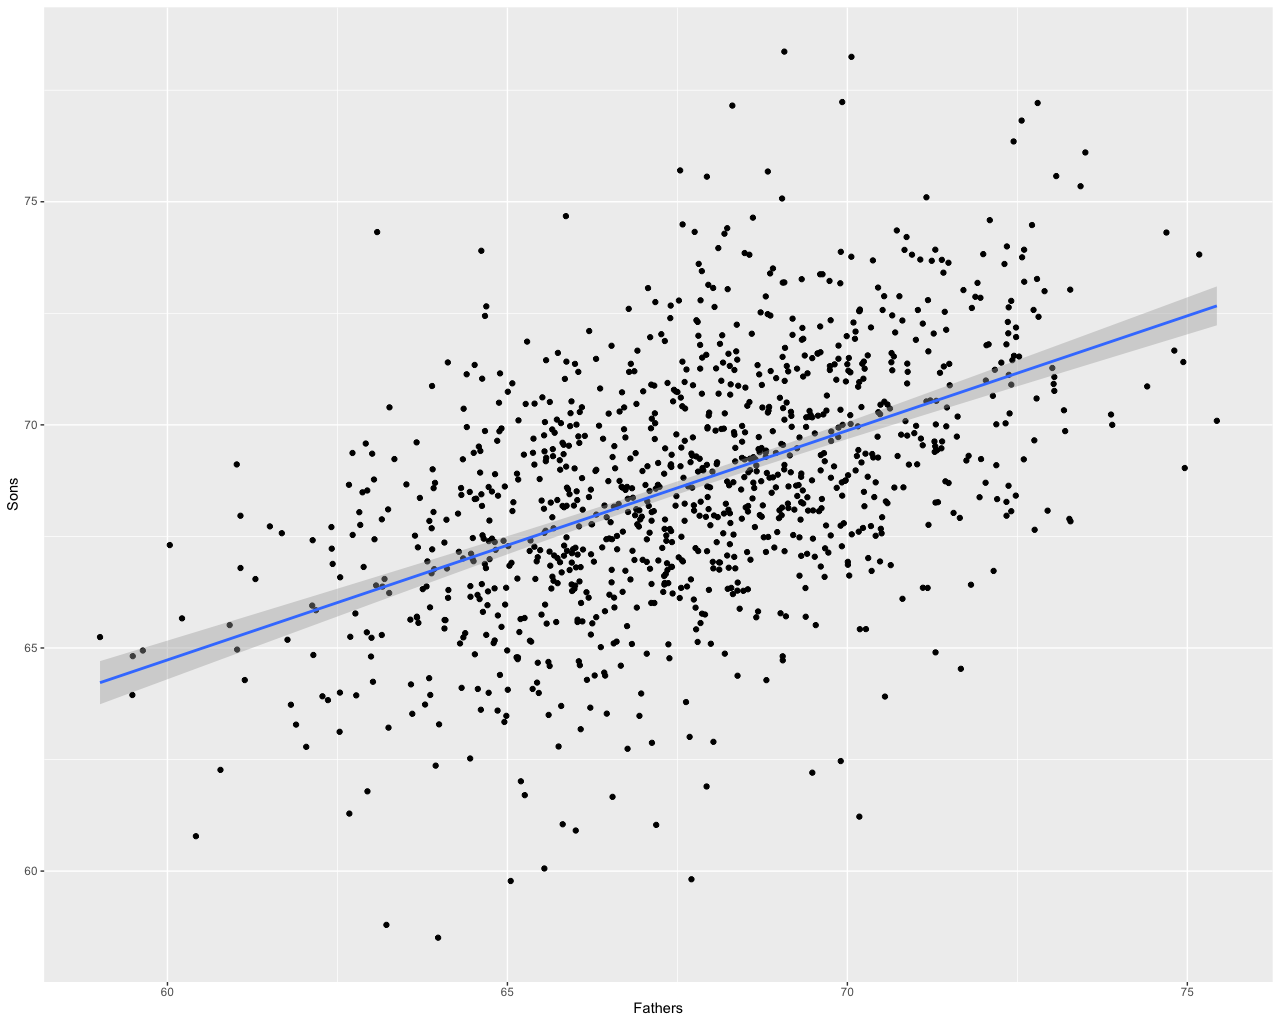
\includegraphics[width=\textwidth,height=0.75\textheight]{pic0059}\end{figure}
\end{frame}

\section{Заключение}

\begin{frame}
\center \huge{Заключение}
\end{frame}

\subsection{Дискусия}

\begin{frame}
\frametitle{Въпроси и отговори}
\center \huge{Благодаря за вниманието!}
\end{frame}

\end{document}
